\chapter{Conclusions}
\label{conclusion}
The proposal describes methods for designing VPNs, while much emphasis is
placed upon the use of structured overlays, much of what described can be used
generically.  The contributions so far describe a scalable, self-configuring,
decentralized VPNs supported by a structured overlay.  Completed components of
this work include:
\begin{itemize}
\item \textbf{Relays} - to enable two-hop connections between peers that cannot
form direct connections.
\item \textbf{Private Virtual Overlays} - secure, self-configuring overlay as
the basis for a structured overlay VPN.
\item \textbf{Group environments} - User-friendly environments to generate
files to ease configuration of complex systems.
\item \textbf{Local VPN configuration} - VPN architect supporting Interface,
Router, and a novel Hybrid mode for various environments.
\end{itemize}

The remaining components of my work are overlay-aware TCP (Chapter~\ref{tcp}),
userspace (socket / HTTP proxy) VPN (Chapter~\ref{userspace_vpn}), and
improving structured P2P VPNs through different usage patterns
(Chapter~\ref{direct_communication}).  For each of these tasks, I will design,
implement, and evaluate the approaches.  The results will lead to new
interesting designs of VPNs using structured overlays.  A schedule for my work
is shown in Figure~\ref{fig:gantt}.

The VPN approaches described herein have been used to construct real systems,
such as the GroupVPN~\cite{gridappliance} and a SocialVPN~\cite{cops08}.  The
GroupVPN has been used to construct a Grid Appliance~\cite{grid_appliance} that
enables the creation of distributed, decentralized, dynamic computing grids.
Over the past 2 years, I have been the student lead in an active grid deployed
for computer architecture research, Archer~\cite{archer}.  Archer currently
spans four universities with 500 resources, we have had 100s of users who
connect seamlessly to these resources from home, school, hotels, etc.  Most
recently, a grid at La Jolla Institute for Allergy and Immunology went live
with minimal communication with our group.  Researchers at the Clemson
University and Purdue have opted for this approach over centralized VPNs as the
basis of their future distributed compute clusters and have actively tested
networks of over 1000 nodes.

\begin{figure}[ht]
\centering
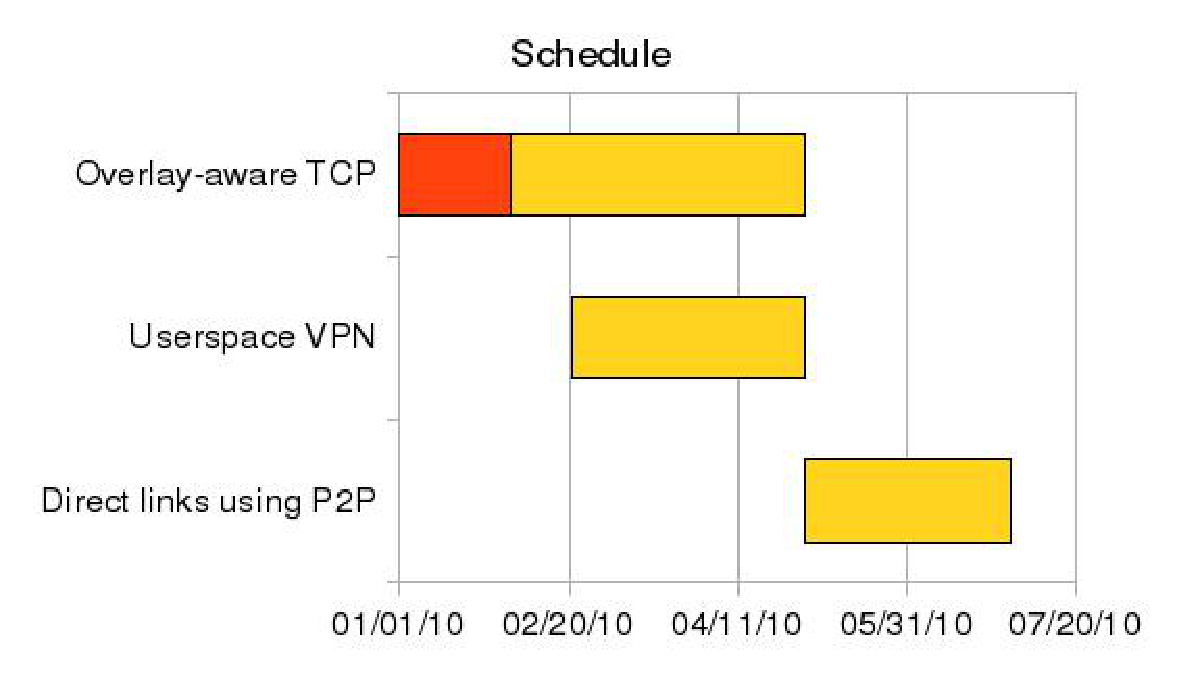
\epsfig{file=figs/schedule.eps, width=4in}
\caption{Schedule for my proposed work.}
\label{fig:gantt}
\end{figure}
